\documentclass[hyperref={pdfpagelabels=false},svgnames]{beamer}
\mode<presentation>{
  \usetheme{Madrid}
  \setbeamertemplate{navigation symbols}{}
}
\usepackage[english]{babel}
\usepackage[latin1]{inputenc}
\usepackage{times}
\usepackage[T1]{fontenc}
\usepackage{graphicx}
\usepackage{tikz}

\title{Operating systems and concurrency - B04}
\subtitle{}
\author{David Kendall}
\institute{Northumbria University}
\date{}
\begin{document}

\begin{frame}
\titlepage
\end{frame}

\begin{frame}
\frametitle{Introduction}
\begin{itemize}
  \item Introduction to threads
  \item Reminder of \texttt{fork()}
  \item \texttt{pthreads} example
  \item Comparison of \texttt{pthreads} with \texttt{fork()}
  \item Main \texttt{pthread} functions
  \item Some problems with threads
\end{itemize}
\end{frame}

\begin{frame}
  \frametitle{What are threads and why do we need them?}
  \begin{itemize}
    \item We have already seen that it is very useful for the OS
      to provide real, or pseudo, concurrency
      \begin{itemize}
        \item We can divide our work up into meaningful units that can
          be considered separately
        \item When some unit of work is blocked waiting for I/O, another unit
          of work can make use of the CPU
      \end{itemize}
    \item So far our unit of work is the \emph{process}
    \item We can create multiple processes and allow the OS to schedule them to 
      maximise the use of resources
    \item But the process is a \emph{heavyweight} unit of work - it comes with
      lots of baggage: in addition to code, static data, registers, stack, heap 
      etc. it also has open files, pipes, signals, sockets, devices etc
    \item The point of \emph{threads} is to give the benefits of concurrency
      but in a much more \emph{lightweight} form
    \item In fact, threads are sometimes called \emph{lightweight processes}
  \end{itemize}
\end{frame}

\begin{frame}
  \frametitle{Single- and multi-threaded processes}
  \begin{center}
    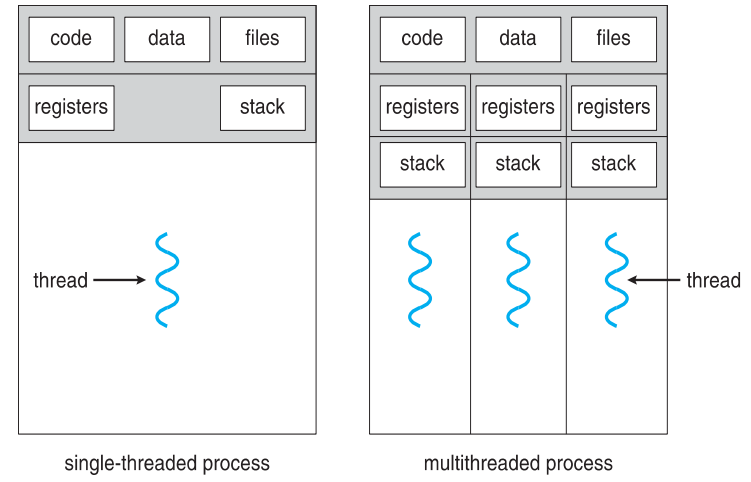
\includegraphics[width=0.6\textwidth]{fig01} \\
    \tiny{Source: SGG12, Chp. 4}
  \end{center}
  \begin{itemize}
    \item On the left is a `standard' process with a 
      single thread of control
    \item On the right is a multi-threaded process --
      a process that has created additional threads
    \item Notice what is shared and what is private
  \end{itemize}
\end{frame}

\begin{frame}[fragile, shrink=10]
  \frametitle{\texttt{fork()} reminder}
  \begin{verbatim}
#include <unistd.h>
#include <stdio.h>
#include <stdlib.h>
#include <sys/wait.h>

int globvar = 6;

int main(void) {
  int var = 88;
  pid_t pid;

  printf("before fork\n");
  if ((pid = fork()) < 0) {
      fprintf(stderr, "fork failed\n");
      exit(-1);
  } else if (pid == 0) {
      globvar++; //child
      var++;
      printf("Child : pid = %d, globvar = %d, var = %d\n",
               getpid(), globvar, var);
  } else {
      waitpid(pid, NULL, 0); // parent
      printf("Parent: pid = %d, globvar = %d, var = %d\n",
               getpid(), globvar, var);
  }
  exit(0);
}
  \end{verbatim}
\end{frame}

\begin{frame}[fragile, shrink=10]
  \frametitle{\texttt{pthreads} example}
  \begin{verbatim}
#include <unistd.h>
#include <stdio.h>
#include <stdlib.h>
#include <pthread.h>

int globvar = 6;

void *threadController(void *arg) {
      globvar++; 
      // var++; Notice this variable is not accessible
      printf("New thread : pid = %d, tid = 0x%lx, globvar = %d, "
              "var = %s\n", getpid(), (unsigned long)pthread_self(),
              globvar, "Not accessible");
      pthread_exit((void *)0);        
}

int main(void) {
  int var = 88;
  pthread_t thread;

  printf("before thread create\n");
  if (pthread_create(&thread, NULL, threadController, NULL) != 0) {
      fprintf(stderr, "thread create failed\n");
      exit(-1);
  } else {
      pthread_join(thread, NULL); // main thread
      printf("Main thread: pid = %d, tid = 0x%lx, globvar = %d, " 
             "var = %d\n", getpid(), (unsigned long)pthread_self(),
              globvar, var);
  }
  exit(0);
}
  \end{verbatim}
\end{frame}

\begin{frame}[fragile]
  \begin{block}{\texttt{fork()} compilation and output}
    \begin{verbatim}
$ gcc -o forkexample1 forkexample1.c
$ ./forkexample1
before fork
Child : pid = 9805, globvar = 7, var = 89
Parent: pid = 9804, globvar = 6, var = 88
    \end{verbatim}
  \end{block}
  \begin{block}{\texttt{pthread} compilation and output}
    \begin{verbatim}
$ gcc -pthread -o threadexample1 threadexample1.c
$ ./threadexample1
before thread create
New thread : pid = 11030, tid = 0x7f12ddb66700, \ 
             globvar = 7, var = Not accessible
Main thread: pid = 11030, tid = 0x7f12de347740, \
             globvar = 7, var = 88
    \end{verbatim}
  \end{block}
\end{frame}


\begin{frame}
  \frametitle{Points to notice in the example}
  \begin{itemize}
    \item \texttt{threadexample} must be compiled with
      the option \texttt{-pthread}
      \begin{itemize}
        \item this links the \texttt{pthread} library into
          the executable
      \end{itemize}
    \item Process identifiers in \texttt{fork} example are
      \emph{different}
    \item Process identifiers in \texttt{pthread} example
      are \emph{the same}
    \item \texttt{globvar} and \texttt{var} in the parent and child
      processes are \emph{separate}
    \item \texttt{globvar} in the main and new threads are \emph{shared}
      \begin{itemize}
        \item \texttt{var} is only accessible in the main thread, not in 
          the new thread
      \end{itemize}
    \item The main and new threads can be distinguished using the
      \emph{thread identifiers} (\texttt{tid})
  \end{itemize}
\end{frame}

\begin{frame}[fragile, shrink=10]
  \frametitle{Thread creation and destruction}
  \begin{itemize}
    \item Create thread
      \begin{verbatim}
#include <pthread.h>
int pthread_create(pthread_t *thread, 
                   const pthread_attr_t *attr,
                   void *(*start_routine) (void *), 
                   void *arg);
Compile and link with -pthread.
      \end{verbatim}
      Creates \verb'thread' with attributes \verb'attr' and
      calls the \verb'start_routine' with argument \verb'arg'
    \item Terminate thread
      \begin{verbatim}
void pthread_exit(void *retval);
      \end{verbatim}
      Can also just \verb'return' from the thread. Terminates the calling
      thread and returns a value that is available to another thread in the same process that
      calls \verb'pthread_join'
  \end{itemize}
\end{frame}

\begin{frame}[fragile]
  \frametitle{Thread join and self}
  \begin{itemize}
    \item Thread join
      \begin{verbatim}
#include <pthread.h>
int pthread_join(pthread_t thread, void **retval);
      \end{verbatim}
      Wait for \verb'thread' to terminate. Return immediately if
      \verb'thread' has already terminated. If \verb'retval' is not
      \verb'NULL' then copy then exit status of the target thread
      into the location pointed to by \verb'*retval'
    \item Thread self
      \begin{verbatim}
pthread_t pthread_self(void);
      \end{verbatim}
      Return the ID of the calling thread. This is the same value
      that is returned in \verb'*thread' in the \verb'pthread_create()' call
      that created this thread
  \end{itemize}
\end{frame}

\begin{frame}
  \frametitle{Threads in action}
  \begin{center}
    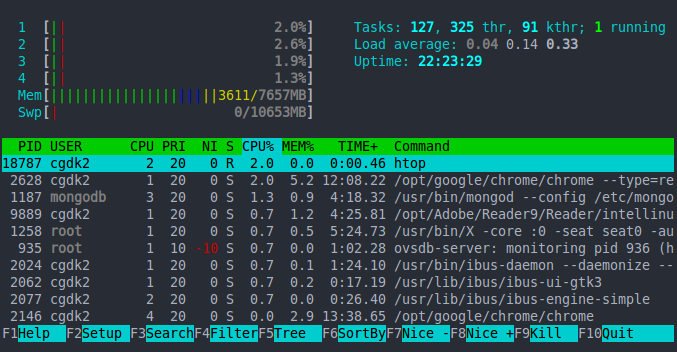
\includegraphics[width=.75\textwidth]{fig02}
  \end{center}
  \begin{itemize}
    \item Output from \texttt{htop}
    \item Shows a machine with 4 cores
    \item Running 127 processes with 325 threads and 91 kernel threads
    \item 1 thread currently running
  \end{itemize}
\end{frame}

\begin{frame}
  \frametitle{Some problems with threads}
  \begin{itemize}
    \item Threads are not without their problems
    \item The main problems arise when multiple threads try
      to access shared data
    \item This can lead to \emph{unpredictable} results
    \item The unpredictability arises because we don't know
      which thread will be chosen by the scheduler to execute
      next
    \item This leads to different instruction sequences
    \item and different instruction sequences can lead to different
      results!
    \item This has given rise to a whole discipline of concurrent programming
      with locks, semaphores, mutexes, condition variables etc. needed to
      recover predictable behaviour
    \item \ldots more on this later in the module
  \end{itemize}
\end{frame}

\end{document}
